\section{Study Settings}

\begin{figure*}[ht]
  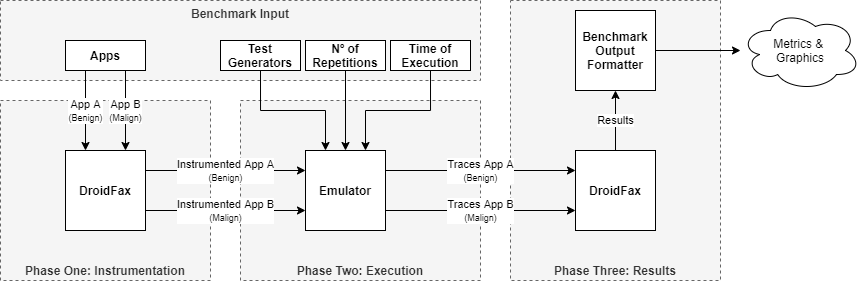
\includegraphics[width=1\textwidth]{images/benchmark3.png}
  \label{benchArq}
  \caption{Benchmark architecture}
  \label{fig:benchArq}
\end{figure*}

In this section, we present the setting of our study, whose main goal is to perform a non-exact replication of the work of Bao et al. and understand the implications of static analysis algorithms in his results. We also investigate how static analysis can improve the performance of testing tools in the task of identifying malicious behaviors.

To achieve this general goal, we answer the following research questions. 

\begin{enumerate}[(RQ1)]
\item What is the effective performance of each tool in terms of the number of detected malware ?
\item What benefits of using a hybrid approach, which combines static and dynamic analysis, for mining sandboxes ?
\item What is the impact of static analysis on benchmark results ?
\end{enumerate}

To assess the effectiveness of mining sandboxes created by each test case generation tools, we used a benchmark solution for test case generation called droidXP \cite{DBLP:conf/scam/CostaMCMVBC20}, that aims us to reproduce previous research work on mining sandboxes. (Figure \ref{fig:benchArq}) show all details of the benchmark architecture used at our experiments. The benchmark run these tools in benign apps and, based on resources sensitives access in this execution, we build their sandbox.

Thereby, to answer the research questions above, we perform two experiments. At both we employed the same dataset, 98 pair of real-world apps (B/M), shared by the AndroZoo \cite{DBLP:conf/msr/AllixBKT16} group. This time we executed each app in one of the five test generator tool, selected for our experiments, for 3 minutes, and for just one time. The droidXP benchmark also relies on DroidFax, the same tool used by Bao et al. in your study, that instruments Android apps and collects relevant information about their execution (using the test case generation tools). DroidFax collects the set of sensitive APIs during a test execution, and during a static analysis at each code apps. Based on this sensitive APIs, that will compose our sandbox, we investigate the capacity of detect malicious behaviors in the corresponding malign app by the tool under analysis, together with the static analysis of the DroidFax. (Figure \ref{fig:setup}) show this experimental setup.

\subsection{First Study: hybrid proposal}

In the first experiment, we executed the benchmark considering the droidXP default configuration, that is, using a hybrid proposal. To generate inputs to apps, we investigate five popular test case generation tools, one from industry (Monkey \cite{Monkey}) and four from academia (Droidbot \cite{DBLP:conf/icse/LiYGC17}, Humanoid \cite{DBLP:conf/kbse/LiY0C19}, DroidMate \cite{DBLP:conf/icse/JamrozikZ16} and ``Joke" tool). This last is a fake tool that we implemented, which does not do anything during the benchmark execution, and through it we can compute results without the dynamic analysis influence. So, we used this experiment to answer the first research questions (RQ1).

\subsection{Second Study: Dynamic analysis proposal}

In this second experiment we used a option of the benchmark that disables the static analysis performed by DroidFax, and with this new configuration, we performed our second study in the same set of apps from the first, at the same execution time, and at the same test case generation tools, including our ``Joke" tool. With the results, it was possible to compute what was the aid portion of the static analysis in the malware detection, since the Joke results, was computed without the dynamic analysis influence. We used this experiment to answer the research questions (RQ2) and (RQ3).


\begin{figure*}[ht]
  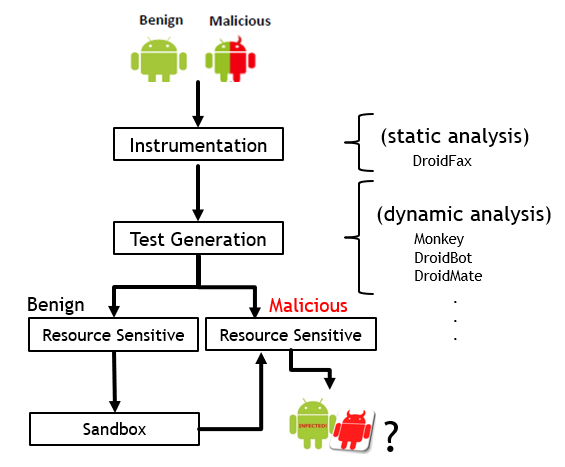
\includegraphics[width=0.5\textwidth]{images/setup.png}
  \label{Experiment setup}
  \caption{Experiment setup}
  \label{fig:setup}
\end{figure*}




